\documentclass{beamer}

\usepackage[T1]{fontenc}
\usepackage[utf8x]{inputenc}

\usepackage{bm}
\usepackage{stmaryrd}
\SetSymbolFont{stmry}{bold}{U}{stmry}{m}{n}

\usepackage{amsmath}
\usepackage{mathtools}

\usepackage{nicematrix}
\definecolor{lblue}{rgb}{.80, .90, .95}
\definecolor{lorange}{rgb}{1, .85, .60}

\usepackage{graphicx}

\usepackage{amsfonts}

\usepackage{color}
\definecolor{keywordcolor}{rgb}{0.7, 0.1, 0.1} % red
\definecolor{commentcolor}{rgb}{0.4, 0.4, 0.4} % grey
\definecolor{symbolcolor}{rgb}{0.0, 0.1, 0.6}  % blue
\definecolor{sortcolor}{rgb}{0.1, 0.5, 0.1}    % green

\usepackage{listings}
\def\lstlanguagefiles{lstlean.tex}
\lstset{language=lean}

\newcommand{\ZZ}{\mathbb{Z}}
\newcommand{\NN}{\mathbb{N}}
\newcommand{\bloch}[2]{\Block[draw=white,fill=lblue,line-width=.5mm,rounded-corners]{#1}{#2}}
\newcommand{\RPP}{\mathsf{RPP}}
\newcommand{\PRF}{\mathsf{PRF}}
\newcommand{\rppId}{\mathsf{Id}}
\newcommand{\rppNe}{\mathsf{Ne}}
\newcommand{\rppSu}{\mathsf{Su}}
\newcommand{\rppPr}{\mathsf{Pr}}
\newcommand{\rppSw}{\mathsf{Sw}}
\newcommand{\rppCo}{\fatsemi}
\newcommand{\rppPa}{\Vert}
\newcommand{\rppIt}{\mathsf{It}}
\newcommand{\rppIf}{\mathsf{If}}

\usetheme{Default}
\usecolortheme{default}
\usefonttheme[onlymath]{serif}

\begin{document}

\begin{frame}
  \begin{itemize}
    \setlength\itemsep{4em} \pause
    \item \textbf{Proof assistant}: software che aiuta nello sviluppo di dimostrazioni formali \pause
    \item \textbf{NON} coincidono con gli automatic theorem prover
  \end{itemize}

\end{frame}

\begin{frame}
  \frametitle{Alcuni traguardi} \pause

  \begin{columns}[onlytextwidth,T]
    \column{30mm}
    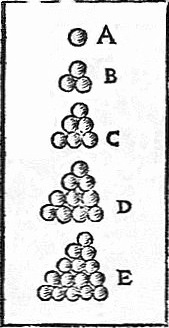
\includegraphics[width=30mm]{kepler.jpg}

    \column{\dimexpr\linewidth-30mm-5mm}
    \begin{itemize}
      \setlength\itemsep{4em}
      \item Congettura di Keplero\\(Thomas Hales, 2015) \pause
      \item \textit{Liquid Tensor Experiment}\\(Peter Scholze, 2021)
    \end{itemize}

  \end{columns}

\end{frame}

\begin{frame}
  \frametitle{Strumenti}
  \begin{center}
\includegraphics[width=0.6\textwidth]{lean.png}\end{center}
  \begin{itemize}
  \setlength\itemsep{2em}
  \item Un proof assistant: Lean Theorem Prover\\(Microsoft Research, 2013) \pause
  \item Una libreria digitalizzata di matematica: Mathlib (2017)
  \end{itemize}
\end{frame}

\begin{frame}
  \frametitle{Soggetto} \pause

  \begin{itemize}
    \setlength\itemsep{4em}
    \item \textit{A class of Recursive Permutations which is Primitive Recursive complete}\\
      (Luca Paolini, Mauro Piccolo, Luca Roversi, 2019) \pause

    \item Computazione reversibile
      \[\begin{NiceMatrix}[nullify-dots]
        \phantom{x}     & \bloch{3-1}{\text{programma}} & \phantom{x}      \\
        \text{input \ } &                               & \text{ \ output} \\
        \phantom{x}     &                               & \phantom{x}      \\
      \end{NiceMatrix}\] \pause

      Nessuna perdita di informazioni!
  \end{itemize}
\end{frame}

\begin{frame}
  \frametitle{$\RPP$}

  \begin{itemize}
    \item \textbf{Reversible Primitive Permutations} ($\RPP$):
      una classe di funzioni $\ZZ^n \to \ZZ^n$ \textbf{calcolabili}, \textbf{reversibili} che è $\PRF$\textbf{-completa}
  \end{itemize}
\end{frame}

\begin{frame}
  \frametitle{$\RPP$}

  Appartengono a $\RPP$:

  \begin{overlayarea}{\textwidth}{0.8\textheight}

    \only<1-5>{\begin{itemize}
      \item<2-5> L'\textbf{identità} $n$-aria
        \[\begin{NiceMatrix}[nullify-dots]
          x_1    & \bloch{3-1}{\rppId_n} & x_1    \\
          \Vdots &                       & \Vdots \\
          x_n    &                       & x_n    \\
        \end{NiceMatrix}\]

      \item<3-5> La funzione \textbf{negazione}
        \[\begin{NiceMatrix}
          x & \bloch{1-1}{\rppNe} & -x \\
        \end{NiceMatrix}\]

      \item<4-5> La funzione \textbf{successore} e \textbf{predecessore}
        \[\begin{NiceMatrix}
          x & \bloch{1-1}{\rppSu} & x+1 \\
        \end{NiceMatrix}
        \hspace{4em}
        \begin{NiceMatrix}
          x & \bloch{1-1}{\rppPr} & x-1 \\
        \end{NiceMatrix}\]

      \item<5> Lo \textbf{swap}
        \[\begin{NiceMatrix}
          x & \bloch{2-1}{\rppSw} & y \\
          y &                     & x \\
        \end{NiceMatrix}\]
    \end{itemize}}

    \only<6-7>{\begin{itemize}
      \item<6-7> La \textbf{composizione in serie} di due $f, g \in \RPP$
        \[\begin{NiceMatrix}[nullify-dots]
          x_1    & \bloch{3-1}{f \rppCo g} & z_1    & \Block{3-1}{=} & x_1    & \bloch{3-1}{f} & y_1    & \bloch{3-1}{g} & z_1    \\
          \Vdots &                         & \Vdots &                & \Vdots &                & \Vdots &                & \Vdots \\
          x_n    &                         & z_n    &                & x_n    &                & y_n    &                & z_n    \\
        \end{NiceMatrix}\]

      \item<7> La \textbf{composizione parallela} di due $f, g \in \RPP$
        \[\begin{NiceMatrix}[nullify-dots]
          x_1    & \bloch{6-1}{f \rppPa g} & z_1    & \Block{6-1}{=} & x_1    & \bloch{3-1}{f} & z_1    \\
          \Vdots &                         & \Vdots &                & \Vdots &                & \Vdots \\
          x_n    &                         & z_n    &                & x_n    &                & z_n    \\
          y_1    &                         & w_1    &                & y_1    & \bloch{3-1}{g} & w_1    \\
          \Vdots &                         & \Vdots &                & \Vdots &                & \Vdots \\
          y_m    &                         & w_m    &                & y_m    &                & w_m    \\
        \end{NiceMatrix}\]
    \end{itemize}}

    \only<8-9>{\begin{itemize}
      \item<8-9> L'\textbf{iterazione finita} di una $f \in \RPP$
        \[\begin{NiceMatrix}[nullify-dots]
          x      & \bloch{4-1}{\rppIt[f]} & x      & \Block{4-1}{=} & x      &                                                                      &                    &                & x      \\  
          x_1    &                        & y_1    &                & x_1    & \bloch{3-1}{f}                                                       & \Block{3-1}{\dots} & \bloch{3-1}{f} & y_1    \\
          \Vdots &                        & \Vdots &                & \Vdots &                                                                      &                    &                & \Vdots \\
          x_n    &                        & y_n    &                & x_n    &                                                                      &                    &                & y_n    \\
                 &                        &        &                &        & \Block{1-3}{\underbrace{\hspace{5.5em}}_{x \text{ volte (se $x > 0$) }}} &                    &                &        \\
        \end{NiceMatrix}\]

      \item<9> La \textbf{selezione} di tre $f, g, h \in \RPP$
        \[\begin{NiceMatrix}[nullify-dots]
          x      & \bloch{4-1}{\rppIf[f, g, h]} & x      \\
          x_1    &                              & y_1    \\
          \Vdots &                              & \Vdots \\
          x_n    &                              & y_n    \\
        \end{NiceMatrix} \quad
        \begin{NiceMatrix}[nullify-dots]
                       &                     &                  \\
        \Block{3-1}{=} & f (x_1, \dots, x_n) & \text{if } x > 0 \\
                       & g (x_1, \dots, x_n) & \text{if } x = 0 \\
                       & h (x_1, \dots, x_n) & \text{if } x < 0 \\
        \CodeAfter
        \SubMatrix\}{2-1}{4-1}\{  
        \end{NiceMatrix}\]
    \end{itemize}}

  \end{overlayarea}

\end{frame}

\begin{frame}
  \frametitle{Proprietà delle $\RPP$}

  \setbeamercovered{transparent}
  \begin{itemize}
    \item<1-2> calcolabili
    \item<3-6> reversibili
    \item<7-8> $\PRF$-completa
  \end{itemize}
  \setbeamercovered{invisible}

  \vspace{1em}

  \begin{overlayarea}{\textwidth}{0.7\textheight}

  \only<2>{
    Possibile arrivare al risultato tramite algoritmo/procedura concreta
  }

  \only<4>{
    Ogni funzione ammette inversa:
    \begin{itemize}
      \item $\rppId_n^{-1} = \rppId_n$
      \item $\rppNe^{-1} = \rppNe$
      \item $\rppSu^{-1} = \rppPr$
      \item $\rppPr^{-1} = \rppSu$
      \item $\rppSw^{-1} = \rppSw$
      \item $(f \rppCo g)^{-1} = g^{-1} \rppCo f^{-1}$
      \item $(f \rppPa g)^{-1} = f^{-1} \rppPa g^{-1}$
      \item ${\rppIt[f]}^{-1} = \rppIt[f^{-1}]$
      \item ${\rppIf[f, g, h]}^{-1} = \rppIf [f^{-1}, g^{-1}, h^{-1}]$
    \end{itemize}
  }

  \only<5>{
    Per esempio, $\big( \rppSw \rppCo (\rppNe \rppPa \rppSu) \big)^{-1} = (\rppNe \rppPa \rppPr) \rppCo \rppSw$:
    \[\begin{NiceMatrix}
      x & \bloch{2-1}{\rppSw} & y & \bloch{1-1}{\rppNe} & - y   \\
      y &                     & x & \bloch{1-1}{\rppSu} & x + 1 \\
    \end{NiceMatrix}\]
  }

  \only<6>{
    Per esempio, $\big( \rppSw \rppCo (\rppNe \rppPa \rppSu) \big)^{-1} = (\rppNe \rppPa \rppPr) \rppCo \rppSw$:
    \[\begin{NiceMatrix}
      x & \bloch{2-1}{\rppSw} & y & \bloch{1-1}{\rppNe} & - y   \\
      y &                     & x & \bloch{1-1}{\rppSu} & x + 1 \\
    \end{NiceMatrix}\]
    \[\begin{NiceMatrix}
      -y  & \bloch{1-1}{\rppNe} & y & \bloch{2-1}{\rppSw} & x\\
      x+1 & \bloch{1-1}{\rppPr} & x &                     & y\\
    \end{NiceMatrix}\]
  }

  \only<8>{
    Sia $F \in \PRF$. \\
    Allora, esiste $g \in \RPP$ che \textbf{codifica} $F$:
    \[\begin{NiceMatrix}[nullify-dots]
      z      & \bloch{3-1}{g} & z + F(\bm{x}) \\
      \bm{x} &                & \bm{x}        \\
      \bm{0} &                & \bm{0}        \\
    \end{NiceMatrix}\]
  }

  \end{overlayarea}
\end{frame}

\begin{frame}[fragile]
  \frametitle{Formalizzazione in Lean} \pause

  La definizione: divisione in \textbf{sintassi} e \textbf{semantica}. \pause

  \begin{itemize}
    \item Sintassi: \lstinline{RPP}

    \begin{center}
      \lstinline{def f  :=  Sw ;; (Ne ‖ Su)  : RPP} \pause
    \end{center}

    \setlength\itemsep{2em}
    \item Semantica: \lstinline{ev : RPP → (list ℤ → list ℤ)} \pause

    \begin{center}
      \lstinline{‹f› : list ℤ → list ℤ}

      \lstinline{‹f› [x, y] = [-y, x+1]}
    \end{center}
  \end{itemize}
\end{frame}

\begin{frame}[fragile]
  \frametitle{Formalizzazione in Lean}

  Principali teoremi: \pause

  \begin{itemize}
    \item Ogni $\RPP$ è invertibile:
    
    \begin{lstlisting}
theorem inv_iff (f : RPP) (X Y : list ℤ) :
  ‹f⁻¹› X = Y ↔ ‹f› Y = X
    \end{lstlisting}

    \item $\PRF$-completezza:
    
    \begin{lstlisting}
theorem completeness (F : ℕ → ℕ) :
  nat.primrec F → ∃ f : RPP, encode F f
    \end{lstlisting}
  \end{itemize}
\end{frame}

\end{document}